\chapter{Results}

In this chapter, we talk about the results. 

\section{Storing moments} \label{sec:storingMoments}

The first thing we analyze is the technique used for storage and subsequent reconstruction of the Fourier coefficients. Specifically, we need to decide how to map wavelengths to a signal from which the coefficients are obtained. As already mentioned in~\cref{par:spectrumToCoefficientConversion}, we have the choice of both \emph{mirroring} and \emph{warping} the signal, which overall creates four options --- using only mirroring, using only warping, using both or using neither, i.e. utilizing the original signal.

To decide which of these options suits our problem the best, we run an experiment in which we compare the original color of a spectral curve with the color of a spectrum obtained by reconstruction from the original curve's coefficients. We use entries from multiple color atlases (such as the Pantone atlas, Munsell Book of Colors and Macbeth Color Checker) and we compute the average and maximum color difference. For these purposes, we use the Delta E error specified in~\cref{deltaE}. Although we state that the Delta 2000 is better, it is not(why? MFO) due to  discontinuities when using gradients

In~\cref{sec:completeMomentError}, we provide all results obtained from these experiments. Note that using $n$ moments requires storing $n+1$ values in case mirroring is used (i.e. the moments are real) and $2n+1$ values otherwise (i.e. the moments are complex). As we are interested in the number of $coefficients$ needed for storage (and for passing to the optimizer) rather than the number of moments, we surmise the contents of~\cref{sec:completeMomentError} in~\cref{table:comparisonMomentTechnique}, where we present the errors according to the number of coefficients.

\begin{table}[t]
	\centering
	\begin{tabular}{crrrrrrrr}
		\toprule
		\multirow{4}{*}{Coefficients} &
		\multicolumn{8}{c}{Methods} \\
		\cmidrule(lr){2-9}
		&\multicolumn{2}{c}{M\&W} &
		\multicolumn{2}{c}{M\&nW} &
		\multicolumn{2}{c}{nM\&W} &
		\multicolumn{2}{c}{nM\&nW}\\
		\cmidrule(lr){2-9}
		& Avg & Max & Avg & Max & Avg & Max & Avg & Max \\
		\cmidrule(lr){1-9}
		1&35.87&114.04&36.2&113.86&35.92&113.97&36.2&113.86\\
		2&21.3&91.19&26.4&99.44&\textemdash&\textemdash&\textemdash&\textemdash\\
		3&1.65&15.09&15.43&68.06&6.54&42.93&13.24&60.23\\
		4&0.86&5.6&9.93&55.67&\textemdash&\textemdash&\textemdash&\textemdash\\
		5&0.54&2.98&4.19&23.53&2.13&17.51&3.7&17.5\\
		6&0.34&2.22&1.19&5.68&\textemdash&\textemdash&\textemdash&\textemdash\\
		7&0.29&2.17&0.77&2.38&1.13&6.87&0.95&5.3\\
		8&0.28&2.03&0.77&1.86&\textemdash&\textemdash&\textemdash&\textemdash\\
		9&0.26&1.95&0.62&1.43&0.97&4.35&0.48&1.96\\
		\bottomrule
	\end{tabular}
	\caption{The average and maximum \emph{Delta E} error originating from round-trips, i.e. from converting spectra to coefficients $c$ and its subsequent reconstruction from $c$. $M$ represents mirroring, $W$ warping, and the symbol $n$ stands for their negation.}
	\label{table:comparisonMomentTechnique}
\end{table}

According to the observation of~\cref{table:comparisonMomentTechnique}, it is clearly beneficial to use both mirroring and warping. However, correct round-trips are not the only factor we need to take into consideration when fitting the cube. We also need to focus on both the \emph{smoothness of the resulting spectra} and the \emph{behavior of the optimizer} under the current technique.

The smoothness of the spectra is especially important for the interpolation process that takes place during the rendering. Interpolating multiple spiky, non-similar spectra would result in similarly uneven spectra, which, in addition to incorrect color, may be susceptible to extreme metameric artifacts.  

The behavior of the optimizer also plays a big role. During the optimization, it takes into account only the resulting RGB of the curve rather than the shape of the curve itself. Therefore, it does not aim for a curve with a similar shape than its neighbor, which may likewise cause issues during the interpolation.

When we fit from the middle, we only aim for the smoothness of the resulting spectra and for the behavior of the optimizer. We therefore want as less coefficients as possible and, as we do not care about round trips, we can use any of the techniques available.


\begin{figure}[t]
	\centering
	\vspace{1em}
	\begin{subfigure}[t]{0.49\textwidth}
		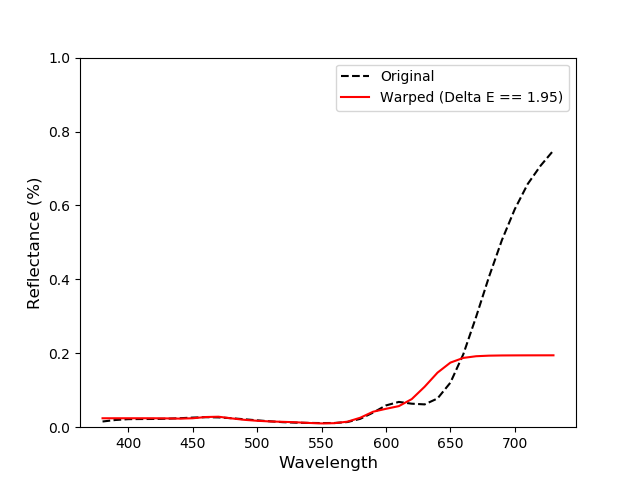
\includegraphics[width=\linewidth]{img/results_worstWarped.png}
		\caption{Warped, Delta E == 1.95, MUNSELL 025R 02 06, 2.5R 2/6 sample }
		\label{fig:resultWorstWarp}
	\end{subfigure} \hspace{0.1em}
	\begin{subfigure}[t]{0.49\textwidth}
		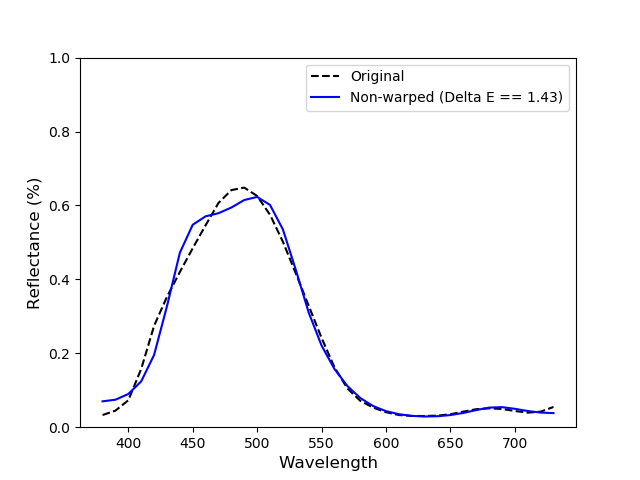
\includegraphics[width=\linewidth]{img/results_worstNonWarped.png}
		\caption{ Pantone 3551 C, Delta E == 1.43}
		\label{fig:resultWorstNonWarp}
	\end{subfigure}
	\caption{Worst case scenarios}
	\label{fig:resultsTechniquesWorst}
\end{figure}


Round trips are important 

This drawback of the optimizer can, for example, be perceived when using warping. As the core idea behind warping is to focus accuracy on the more ``important'' regions of the curve (i.e. around the 550nm wavelength), the reconstruction of the curve's edges is deemed to fail. Moreover, it amplifies the slight bumps that sometimes occur around the middle. This is a desired behavior when we are aiming for correct color reconstruction. However, if we were to use such a curve as prior to a lattice point with similar RGB, we would require only slight changes in its shape, e.g. minor tweaks at the edges of the curve. This, however, is not possible to do when using warping, as this method trades off the capability to influence edges with having too much freedom around the middle. The optimizer is therefore apt to amplify the already existing bumps even more in order to achieve the desired RGB value.

In figure 2, we present the curves reconstructed from the coefficients of the lattice point with the target RGB of (). Both figures 

In a, the cube was fitted from the middle by using the warping technique, while the cube in b did not use warping. For both fittings, we used 9 coefficients and we  We can see that by the time the cube grew enough so that the lattic



 Determining whether to use warp is a bit more complicated.~\citet{trigonometricMomentsPaper} recommend using warping at all times, especially if the number of moments is below 5. The table suggests that although warping results in a higher average error, the maximum error is lower. As we place greater importance on minimizing the maximum error, we are inclined to use warping.

However, warping does not perform as well in terms of curve reconstruction. As its core idea is to focus accuracy on the more ``important'' regions of the curve (i.e. around the 550nm wavelength), it does not reconstruct the edges at all. 




Warping obviously provides better color reconstruction. We lose information in the edges (PICTURE), but that does not matter in terms of color reconstruction. More coefficients can then be focused on the middle, which makes us able to simulate the shape in the middle more accurately, we can e.g. see some slight curves that we cannot do with the same number of moments without warping (PICTURE). (mozeme naznacit ze to z sekcie jedna metamerizmus je warping)

However, as we put a lot of attention to the middle, we therefore allow coefficients to create some extremely crazy shapes. show PICTURE. It does not work well with the optimizer - the optimizer gets prior coefficients, which are fixating on the middle and the optimizer does not care about the shape of the curve but only about the resulting RGB. Therefore, it always zvyrazni, zvacsi the effects of the coefficients (the slight curves that they create). We can see this in picture daco.

Therefore, we do not use warping. We use mirroring - non-mirroring would make us use only a little number of coefficients, which is nevyhodne. 

\section{Number of moments}

For middle fitting, we always recommend 2 moments, 3 coeffs due to the runtime. Moreover, they are very smooth but not straight which is ideal for our purposes. Obviously, we can fit with higher but that takes a lot of time and does not provide any advantage. The default setting is therefore 3 coefs, 2 moments.

Obviously, fitting with these causes metameric artifacts, similar to the ones created by sigmoid, we show these in PICTURE. We can also show metameric artifacts when fitting with more? (try this maybe)

Therefore, we go for fitting with an atlas. The more coefficients, the better the reconstruction when saving an atlas entry. However, we must remind that we do not need to only save the coefs, we need to do the following things:
- create coefficients from atlas entry
- find lattice point closest to atlas entry
- use these coefs as prior for optimizer
- run the optimizer
This already suggests that the optimizer might be the problem, and it is. Imagine we have only an 8-dimensional cube, and the atlas entry is in the middle of voxel. The euclidean distance could be as high as daco, which is too far. Optimizer sice takes the coefficients, but has to change them way too much so they fit what it wants to do. This results in extreme changes and the information from the atlas entry is not utilized at all. We show this in PICTURE.

Our only way ako to obist je proste pouzit a larger cube. Another slight trick is to use a lower number of coefficients - we therefore do not get as big artifacts because we cannot possibly reconstruct such crazy spectra with low number of coefficients. 

TOTO Kludne spomenut aj inde!!! The optimizer is always faster for lower number of coefficients as it does not need to change them up as much. Also faster but does not change them so much SO it results in spectrum that is similar to the first one. However, we cannot possibly simulate the curve with only the limited number of coefficients, the table says so. Therefore we must find something in the middle. We try not to focus on performance here because obviously, fitting anything that is higher than 32 takes hours and we want to have it look the best way we can.




What I did so far:
- created the support for multiple coefficients
- added warping to the signal because the results are definitely better with warping
- however, the problem occurs when we need to actually fit the points - e.g. even if we are using a 32 dimensional cube, white atlas entry of the macbeth is basically right in the middle of the voxel and therefore is far away
- the coefficients that we used to save the curve do not reconstruct the curve exactly but that does not cause problem, the optimizer does
- by saving the signal of white with 9 coefficients WITH warping, the optimizer actually has a lot of work to fit especially the stuff in the middle of voxel -> the resulting curve is way different from the one that we started with, with a lot of sharp things, which cause a lot of metameric artifacts
- if using warping, it is strongly recommended then to use a lot less moments as they force the curve to be smooth and the limited curves help in this case
- we can show some of the results with warping, obviously they suck


We talk about the following results:

- the quality of the fitting - i.e. how many times we get stuck in local minima, how does that behave,

- how many moments should we be using (input the table that we have already created) - we say how many moments we actually support, also mention we could support more (more residual blocks in optimizer) but that would take way too long

- the results when fitting from the middle



- performance of the optimizer

- the quality of the fitting (how far away do we fit, )


Problems with the optimizer:

It can get stuck in local minima, which usually happens in three cases and in combination of them:
- threshold - we cannot control this
- number of coefficients - the lower the better
- cube dimension - the higher the better
We tested this stucking in both when fitting lattice points, where it is crucial (we therefore added a heuristic and tested how often we get in the heuristic):

\begin{figure}[t]
	\centering
	\vspace{1em}
	\begin{subfigure}[t]{0.49\textwidth}
		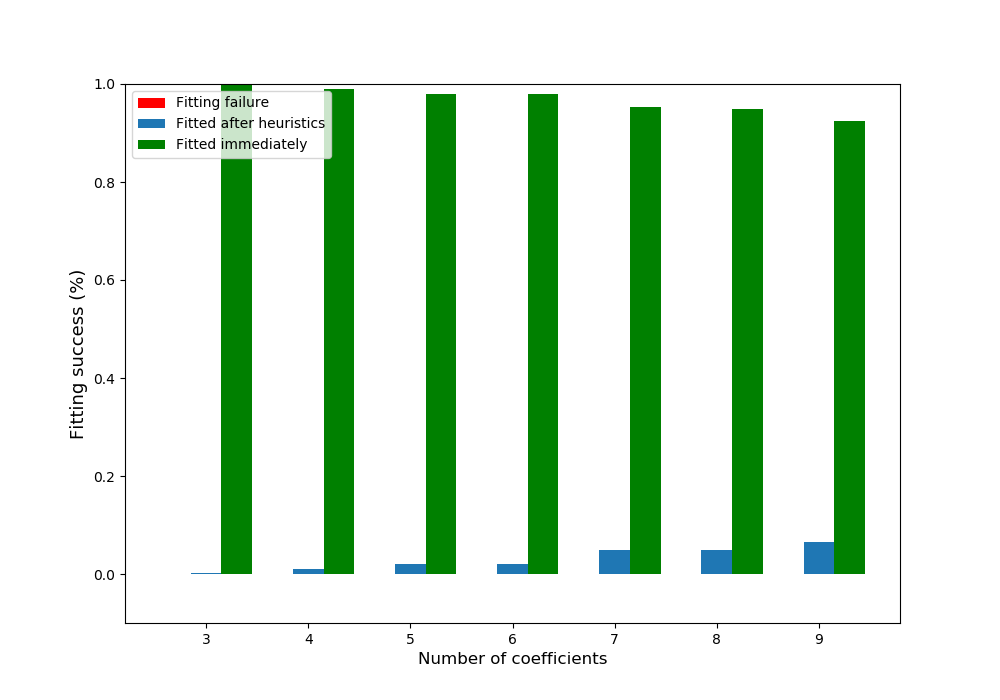
\includegraphics[width=\linewidth]{img/results_perf_fitting_cd16.png}
		\caption{Examples of reconst}
		\label{fig:mom}
	\end{subfigure} \hspace{0.1em}
	\begin{subfigure}[t]{0.49\textwidth}
		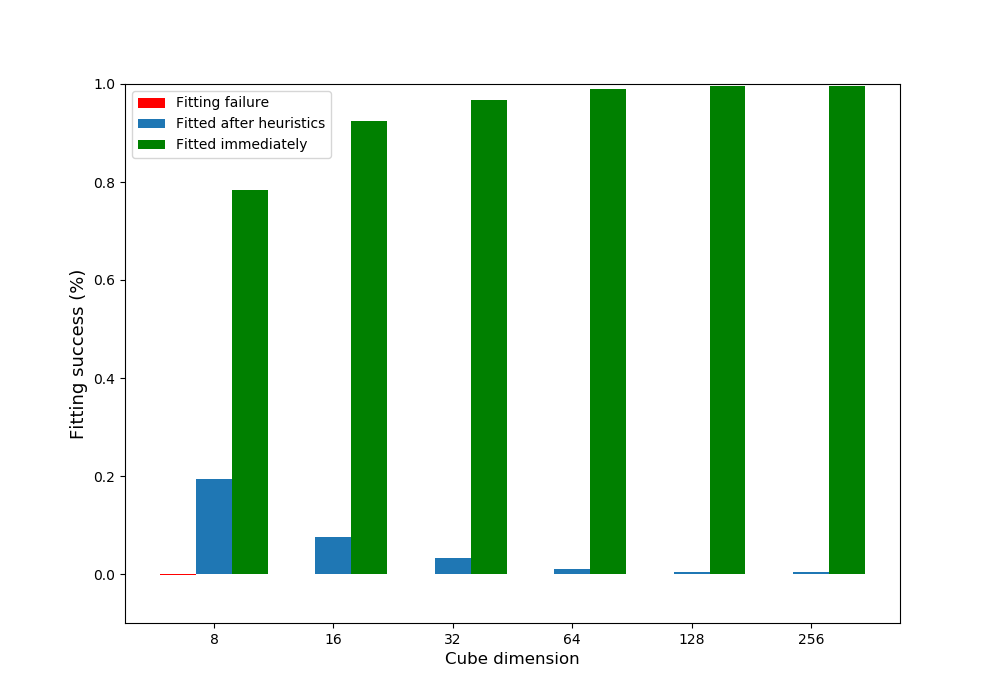
\includegraphics[width=\linewidth]{img/results_perf_fitting_9moments.png}
		\caption{Reconstru.}
		\label{fig:m}
	\end{subfigure}
	\caption{Exampod.}
	\label{fig:temp}
\end{figure}


- for 9 moments (using the 4 atlases, Munsell Book of Colours, RAL, Macbeth color checker, Macbeth Color Checker SG):
	- cd 8 = 1 absolutely not fitted, 355 overall, 278 were fitted immediately, 69 after first,
	8 required second -> 19.44 percent therefore after first, 78.3 percent immediately, 2.2 percent after second 
	
	- cd 16 = all fitted, 851 overall, 787 fitted immediately (92.47 percent), 56 after first (6.58 percent), 8 required second (0.9 percent)
	
	- cd 32 = all fitted (1389), 1344 fitted immediately, 43 fitted after first, 2 required second
	
	- cd 64 = all fitted, 1648 fitted immediately, 15 fitted after first, 2 required second
	 
	 -cd 128 - 1861 fitted immediately, 8 fitted after first, no second
	 
	 -cd 256 - 1911 fitted immediately, 8 fitted after first, no second 
	 
- for 6 moments:
	- cd 8 = all fitted, 355 overall, 326 fitted immediately (91.83 percent), 29 after first (8.16 percent), none required second
	
- for 3 moments:
	- cd 8 = all fitted, 355 overall, 352 fitted immediately (99 percent), 3 after first (1 percent), none required second 
	
	- cd 16 = all fitted, 851 overall, 849 fitted immediately, 2 after first
	
	- cd 32 = all fitted immediately, 

Other moments for cd16:
9: 787 fitted immediately (92.47 percent), 56 after first (6.58 percent), 8 required second (0.9 percent)
8: 809 fitted immediately, 40 after first, 2 after second
7: 1 unfitted at all, 810 immediately, 39 after first, 2 after second
6: all fitted, 833 immediately, 18 after first, 0 after second
5: 833 immediately, 18 after first
4: 842 fitted immediately, 6 after first, 3 after second
3: 849 fitted immediately, 2 after first

	
We also tested stucking in the normal fitting. 


Also mention that it is multi-threaded and performance is not really a priority - the cube has to be created only once and then can be reused as much as the artists need.
